\documentclass{aastex62}   	% use "amsart" instead of "article" for AMSLaTeX format
\usepackage{graphicx}				% Use pdf, png, jpg, or eps§ with pdflatex; use eps in DVI mode
								% TeX will automatically convert eps --> pdf in pdflatex		
\usepackage{amssymb}
\usepackage{natbib}

%SetFonts

%SetFonts

\begin{document}


\subsection{Peculiar Velocities with SNe~Ia}
Peculiar velocities provide a measure of $f\sigma_8$, which in turn probes gravity.  As precise distance indicators Type~Ia supernovae (SNe~Ia)
can provide precise peculiar velocities of their host galaxies \citep{2006PhRvD..73l3526H,2011ApJ...741...67D}.

\citet{2017ApJ...847..128H} calculated the  expected precision of $f\sigma_8$ using LSST-discovered SNe~Ia.
The Fisher information matrix of a random Gaussian field with mean zero and covariance $C(k)$ parameterized by $\lambda$ is
\begin{equation}
F_{ij} = \frac{V}{2}\int \frac{d^3k}{(2\pi)^3} \text{Tr}\left[ C^{-1} \frac{\partial C}{\partial \lambda_i} C^{-1}
\frac{\partial C}{\partial \lambda_j} \right].
\end{equation}
The covariance
\begin{equation}
C = P_{vv}(k) + \frac{\sigma^2}{n}
\end{equation}
has contributions from the power spectrum, noise in the velocity measurement, and the density of velocity probes.
In the sample variance limit for a sample with fixed depth, the variance in $f\sigma_8$ (and other $\lambda$ parameters)
is thus inversely proportional to the survey solid-angle $\Omega$, whereas
in the shot-noise limit the variance is inversely proportional to $\Omega n^2 \propto N^2/\Omega$, where $n$ is the number density,
and $N$ is the total number of supernovae.  

N.~Regnault kindly provided us with his assessment of the number and solid-angle of $z<0.2$ supernova pre-maximum discoveries 
for the survey candidates provided by the Project.  Based on these numbers we calculate the Figures of Merit in the two regimes 
(normalized with respect to the average of all the surveys),
with our results shown in 
Table~\ref{table:ref}.  The results of \citet{2017ApJ...847..128H}  indicate that after 10 years,
LSST supernovae are at neither extreme; we thus adopt the average of the two FoM's as what we advocate for the survey.
These averages for a select set of surveys are shown in Figure~\ref{fig:fom}.


\begin{table}
\caption{SN~Ia Figures of Merit of Project survey candidates
in  the shot-noise and the survey-variance limits.  The final column is the average
of the two Figures of the Merit.\label{table:ref}}
\centering
\begin{tabular}{|c|rrr|}
\hline
Survey & FoM (shot) & FoM (survey) & FoM (avg)\\
\hline
alt\_sched  & 2.788 & 0.910 & 1.849  \\
alt\_sched\_rolling  & 0.804 & 0.920 & 0.862  \\
alt\_sched\_twi  & 2.816 & 0.927 & 1.871  \\
altsched\_18\_\_90\_30  & 2.581 & 1.187 & 1.884  \\
altsched\_18\_\_90\_40  & 2.594 & 1.187 & 1.890  \\
altsched\_good\_weather  & 2.914 & 0.910 & 1.912  \\
altsched\_rolling\_good\_weather  & 0.815 & 0.920 & 0.868  \\
baseline2018a  & 0.779 & 0.834 & 0.807  \\
blobs\_mix\_zmask10yrs  & 1.432 & 1.008 & 1.220  \\
blobs\_same\_10yrs  & 0.064 & 0.859 & 0.462  \\
blobs\_same\_zmask10yrs  & 0.048 & 0.859 & 0.453  \\
cadence\_mix\_10yrs  & 1.012 & 1.012 & 1.012  \\
colossus\_2664  & 0.814 & 0.884 & 0.849  \\
colossus\_2665  & 0.797 & 0.861 & 0.829  \\
colossus\_2667  & 2.365 & 1.004 & 1.684  \\
feature\_baseline\_10yrs  & 0.025 & 0.642 & 0.334  \\
feature\_rolling\_half\_mask\_10yrs  & 0.175 & 0.987 & 0.581  \\
feature\_rolling\_twoThird\_10yrs  & 0.187 & 1.104 & 0.645  \\
kraken\_2026  & 0.947 & 0.838 & 0.892  \\
kraken\_2035  & 0.705 & 0.823 & 0.764  \\
kraken\_2036  & 0.437 & 1.141 & 0.789  \\
kraken\_2042  & 0.794 & 0.858 & 0.826  \\
kraken\_2044  & 2.565 & 1.162 & 1.863  \\
minion\_1016  & 0.093 & 1.109 & 0.601  \\
mothra\_2045  & 0.226 & 1.134 & 0.680  \\
mothra\_2049  & 0.671 & 1.161 & 0.916  \\
nexus\_2097  & 0.280 & 1.166 & 0.723  \\
pontus\_2002  & 0.224 & 1.157 & 0.691  \\
pontus\_2489  & 2.052 & 0.970 & 1.511  \\
pontus\_2502  & 0.132 & 1.107 & 0.620  \\
rolling\_10yrs  & 0.581 & 0.838 & 0.709  \\
rolling\_mix\_10yrs  & 0.958 & 1.011 & 0.984  \\
rolling\_mix\_75\_10yrs  & 0.850 & 1.007 & 0.928  \\
tight\_mask\_10yrs  & 0.646 & 1.155 & 0.901  \\
tight\_mask\_simple\_10yrs  & 0.600 & 1.141 & 0.871  \\
tms\_drive\_10yrs  & 0.806 & 1.090 & 0.948  \\
tms\_roll\_10yrs  & 0.424 & 1.119 & 0.771  \\
\hline
\end{tabular}
\end{table}

\begin{figure}[htbp]
   \centering
   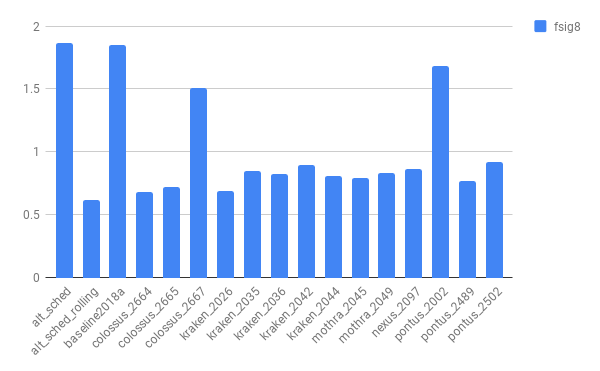
\includegraphics[scale=0.5]{chart.png} % requires the graphicx package
   \caption{Figure of Merits of Select Surveys}
   \label{fig:fom}
\end{figure}

We are in the course of refining the Figure or Merit, taking into account survey geometry, combining both survey variance and shot noise.
Any significant changes in our findings will lead to an update of our relative
ranking of the surveys.


\begin{thebibliography}{}
\expandafter\ifx\csname natexlab\endcsname\relax\def\natexlab#1{#1}\fi
\providecommand{\url}[1]{\href{#1}{#1}}
\providecommand{\dodoi}[1]{doi:~\href{http://doi.org/#1}{\nolinkurl{#1}}}
\providecommand{\doeprint}[1]{\href{http://ascl.net/#1}{\nolinkurl{http://ascl.net/#1}}}
\providecommand{\doarXiv}[1]{\href{https://arxiv.org/abs/#1}{\nolinkurl{https://arxiv.org/abs/#1}}}

\bibitem[Davis et al.(2011)]{2011ApJ...741...67D} Davis, T.~M., Hui, L., Frieman, J.~A., et al.\ 2011, \apj, 741, 67.  
\bibitem[Hui, \& Greene(2006)]{2006PhRvD..73l3526H} Hui, L., \& Greene, P.~B.\ 2006, \prd, 73, 123526.
  
\bibitem[Howlett et al.(2017)]{2017ApJ...847..128H} Howlett, C., Robotham, A.~S.~G., Lagos, C.~D.~P., et al.\ 2017, \apj, 847, 128.
\end{thebibliography}
\bibliographystyle{plainnat}
\end{document}  